\documentclass[12pt]{article}

%%%%%%%%%%%%%%%%%%%%%%%%%%%%%%%%%%%%%%%%%%%%%%%%%%%%%%%%%%%%%%%%%%%%%%%%%%%%%%%%
%                           Package preset for homework
%%%%%%%%%%%%%%%%%%%%%%%%%%%%%%%%%%%%%%%%%%%%%%%%%%%%%%%%%%%%%%%%%%%%%%%%%%%%%%%%
% Miscellaneous
\usepackage[margin=1in]{geometry}
\usepackage[utf8]{inputenc}
\usepackage{indentfirst}
\usepackage{blindtext}
\usepackage{graphicx}
\usepackage{xr-hyper}
\usepackage{hyperref}
\usepackage{enumitem}
\usepackage{color}
\usepackage{float}
% Math
\usepackage{latexsym}
\usepackage{amsfonts}
\usepackage{amssymb}
\usepackage{amsmath}
\usepackage{commath}
\usepackage{amsthm}
\usepackage{bbold}
\usepackage{bm}
% Physics
\usepackage{physics}
\usepackage{siunitx}
% Code typesetting
\usepackage{listings}
% Citation
\usepackage[authoryear]{natbib}
\usepackage{appendix}
\usepackage[capitalize]{cleveref}
% Title & name
\title{Homework}
\author{Tien Vo}
\date{\today}


%%%%%%%%%%%%%%%%%%%%%%%%%%%%%%%%%%%%%%%%%%%%%%%%%%%%%%%%%%%%%%%%%%%%%%%%%%%%%%%%
%                   User-defined commands and environments
%%%%%%%%%%%%%%%%%%%%%%%%%%%%%%%%%%%%%%%%%%%%%%%%%%%%%%%%%%%%%%%%%%%%%%%%%%%%%%%%
%%% Misc
\sisetup{load-configurations=abbreviations}
\newcommand{\due}[1]{\date{Due: #1}}
\newcommand{\hint}{\textit{Hint}}
\let\oldt\t
\renewcommand{\t}[1]{\text{#1}}

%%% Bold sets & abbrv
\newcommand{\N}{\mathbb{N}}
\newcommand{\Z}{\mathbb{Z}}
\newcommand{\R}{\mathbb{R}}
\newcommand{\Q}{\mathbb{Q}}
\let\oldP\P
\renewcommand{\P}{\mathbb{P}}
\newcommand{\LL}{\mathcal{L}}
\newcommand{\FF}{\mathcal{F}}
\newcommand{\HH}{\mathcal{H}}
\newcommand{\NN}{\mathcal{N}}
\newcommand{\ZZ}{\mathcal{Z}}
\newcommand{\RN}[1]{\textup{\uppercase\expandafter{\romannumeral#1}}}
\newcommand{\ua}{\uparrow}
\newcommand{\da}{\downarrow}

%%% Unit vectors
\newcommand{\xhat}{\vb{\hat{x}}}
\newcommand{\yhat}{\vb{\hat{y}}}
\newcommand{\zhat}{\vb{\hat{z}}}
\newcommand{\nhat}{\vb{\hat{n}}}
\newcommand{\rhat}{\vb{\hat{r}}}
\newcommand{\phihat}{\bm{\hat{\phi}}}
\newcommand{\thetahat}{\bm{\hat{\theta}}}

%%% Other math stuff
\providecommand{\units}[1]{\,\ensuremath{\mathrm{#1}}\xspace}
% Set new style for problem
\newtheoremstyle{problemstyle}  % <name>
        {10pt}                   % <space above>
        {10pt}                   % <space below>
        {\normalfont}           % <body font>
        {}                      % <indent amount}
        {\bfseries\itshape}     % <theorem head font>
        {\normalfont\bfseries:} % <punctuation after theorem head>
        {.5em}                  % <space after theorem head>
        {}                      % <theorem head spec (can be left empty, 
                                % meaning `normal')>

% Set problem environment
\theoremstyle{problemstyle}
\newtheorem{problemenv}{Problem}[section]
\newenvironment{problem}[1]{%
  \renewcommand\theproblemenv{#1}%
  \problemenv
}{\endproblemenv}
% Set lemma environment
\newenvironment{lemma}[2][Lemma]{\begin{trivlist}
\item[\hskip \labelsep {\bfseries #1}\hskip \labelsep {\bfseries #2.}]}{\end{trivlist}}
% Set solution environment
\newenvironment{solution}{
    \begin{proof}[Solution]$ $\par\nobreak\ignorespaces
}{\end{proof}}
\numberwithin{equation}{problemenv}

%%% Page format
\setlength{\parindent}{0.5cm}
\setlength{\oddsidemargin}{0in}
\setlength{\textwidth}{6.5in}
\setlength{\textheight}{8.8in}
\setlength{\topmargin}{0in}
\setlength{\headheight}{18pt}

%%% Code environments
\definecolor{dkgreen}{rgb}{0,0.6,0}
\definecolor{gray}{rgb}{0.5,0.5,0.5}
\definecolor{mauve}{rgb}{0.58,0,0.82}
\lstset{frame=tb,
  language=Python,
  aboveskip=3mm,
  belowskip=3mm,
  showstringspaces=false,
  columns=flexible,
  basicstyle={\small\ttfamily},
  numbers=none,
  numberstyle=\tiny\color{gray},
  keywordstyle=\color{blue},
  commentstyle=\color{dkgreen},
  stringstyle=\color{mauve},
  breaklines=true,
  breakatwhitespace=true,
  tabsize=4
}
\lstset{
  language=Mathematica,
  numbers=left,
  numberstyle=\tiny\color{gray},
  numbersep=5pt,
  breaklines=true,
  captionpos={t},
  frame={lines},
  rulecolor=\color{black},
  framerule=0.5pt,
  columns=flexible,
  tabsize=2
}


\title{Final: Astr 5140 (Fall 2021)}

\begin{document}
\maketitle
%%%%%%%%%%%%%%%%%%%%%%%%%%%%%%%%%%%%%%%%%%%%%%%%%%%%%%%%%%%%%%%%%%%%%%%%%%%%%%%
\begin{problem}{1}[Particle Motion in a Gravitational Field]
Examine the diagram below. A plasma in a gravitational field ($x$ direction) is
supported by a magnetic field ($B_z$) in the $z$ direction. Set $\vb{E}=\vb{0}$.

\begin{center}
    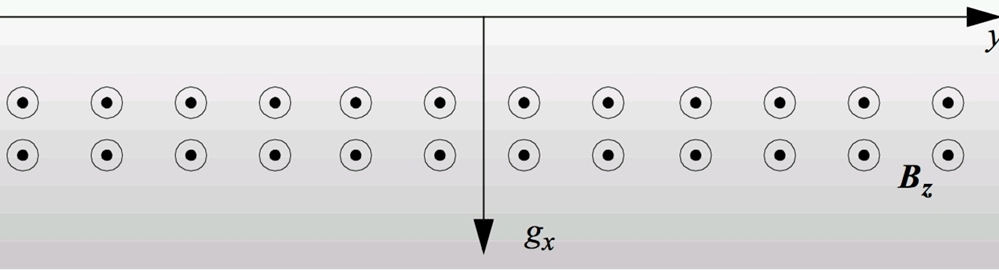
\includegraphics[width=0.7\textwidth]{final_p1.jpg}
\end{center}

(a) Start with the basic equations of motion of a charged particle in a magnetic
field $\vb{v}=v_x(t)\xhat+v_y(t)\yhat$ and gravitational force. Break the
Lorentz equation into its components,
\begin{equation}
    \frac{\partial v_x}{\partial t}=\frac{qB_z}{m}v_y+g
    \qquad\text{and}\qquad
    \frac{\partial v_y}{\partial t}=-\frac{qB_z}{m}v_x
\end{equation}
where $\vb{B}=B\zhat$. Average over time (alternatively, ignore gyration) to
arrive at the gravitational drift.

(b) Calculate the current $\vb{J}$ for a constant plasma density $\rho_0$.

(c) Show that the current from gravitational drift is equivalent to that in the
MHD force equation.

(d) Setting the single fluid velocity to $\vb{u}\approx \vb{v}_{Di}$, is
$\vb{E}+\vb{u}\times\vb{B}=0$? ($\vb{v}_{Di}$ is the ion gravitational drift).

(e) Show generalized Ohm's law must include the Hall term to be consistent with
the gravitational drift in the limit of $m_i\gg m_e$. Should Hall MHD be used in
the presence of strong gravitational field?
\begin{solution}
(a) Given $\vb{g}=g\xhat$ and $\vb{B}=B\zhat$, the force equation is
\begin{equation}
    m\frac{d\vb{v}}{dt}=m\vb{g}+q\vb{v}\times\vb{B}\Rightarrow
    \vb{v}=g\xhat+\Omega_c(v_y\xhat-v_x\yhat)
\end{equation}
where we have written $\Omega_c=qB/m$. So the velocity components satisfy the
following differential equations
\begin{equation}
    \dot{v}_x=g+\Omega_cv_y\qquad\text{and}\qquad
    \dot{v}_y=-\Omega_cv_x
\end{equation}
Taking another time derivative and combining the two equations, we get the
following differential equation for $v_x$
\begin{equation}
    \ddot{v}_x=\Omega_c\dot{v}_y=-\Omega_c^2v_x 
\end{equation}
The general solution for $v_x$ is
\begin{equation}
    v_x=v_\perp \cos\qty(\Omega_ct+\delta)    
\end{equation}
where $v_\perp,\delta$ are initial conditions dependent constants. We can
then find $v_y$
\begin{equation}
    v_y=\frac{\dot{v}_x}{\Omega_c}-\frac{g}{\Omega_c}=
    -v_\perp\sin\qty(\Omega_ct+\delta)-\frac{g}{\Omega_c}
\end{equation}
Averaging over one period, $\expval{\sin(\Omega t+\delta)}=0$, so there remains
a drift in the $y$ direction
\begin{equation}
    v_D=\expval{v_y}=-\frac{g}{\Omega_c} 
\end{equation}
So the gravitational drift is
\begin{equation}\label{p1a:vd}
    \vb{v}_D=-\frac{g}{\Omega_c}\yhat=\frac{m}{q}\frac{\vb{g}\times\vb{B}}{B^2}
    =-\frac{mg}{qB}\yhat
\end{equation}

(b) The current due to the electron drift is
\begin{equation}
    \vb{J}_{e}=-ne\vb{v}_{De}=nm_e\frac{\vb{g}\times\vb{B}}{B^2}
\end{equation}
and the current due to the ion drift is
\begin{equation}
    \vb{J}_i=ne\vb{v}_{Di}=nm_i\frac{\vb{g}\times\vb{B}}{B^2} 
\end{equation}
Thus, the total current is
\begin{equation}
    \vb{J}=\vb{J}_i+\vb{J}_e=n(m_e+m_i)\frac{\vb{g}\times\vb{B}}{B^2}
    =\rho_0\frac{\vb{g}\times\vb{B}}{B^2}
    =-\frac{\rho_0g}{B}\yhat
\end{equation}

(c) Recall that the current in the force equation $\vb{J}\times\vb{B}$ comes
from the term
\begin{equation}
    n_sq_s\vb{u}_s\times\vb{B} 
\end{equation}
in the two-fluid equations where $\vb{u}_s$ is the drift of the particle
species. Here, the only drift is due to gravitation. Thus, by definition,
$\vb{J}=\sum_sn_sq_s\vb{u}_s$ in the force equation is the same as that in part 
(b).

(d) Since $\vb{u}=\vb{v}_{Di}$, from \eqref{p1a:vd},
\begin{equation}\label{p1d:ohm}
    \vb{E}+\vb{u}\times\vb{B}=-\frac{m_ig}{e}\yhat\times\zhat=-\frac{m_ig}{e}\xhat
    \neq0
\end{equation}
where $M$ is the ion mass.

(d) By definition, the Hall term is
\begin{equation}
    \frac{\vb{J}\times\vb{B}}{ne}
    =-\frac{\rho_0g}{ne}\yhat\times\zhat
    =-\frac{\rho_0g}{ne}\xhat
\end{equation}
But $\rho_0\approx nm_i$ when $m_i\gg m_e$, so
\begin{equation}
    \frac{\vb{J}\times\vb{B}}{ne}=-\frac{m_ig}{e}\xhat 
\end{equation}
This is the same as the RHS in \eqref{p1d:ohm}. So we must require that the
generalized Ohm's law have the Hall term
\begin{equation}
    \vb{E}+\vb{u}\times\vb{B}=\frac{\vb{J}\times\vb{B}}{ne} 
\end{equation}
In the presence of strong gravitational field, Hall MHD should be used because
the plasma is certainly not ideal, as indicated by part (d).
\end{solution}
\end{problem}
%%%%%%%%%%%%%%%%%%%%%%%%%%%%%%%%%%%%%%%%%%%%%%%%%%%%%%%%%%%%%%%%%%%%%%%%%%%%%%%
%%%%%%%%%%%%%%%%%%%%%%%%%%%%%%%%%%%%%%%%%%%%%%%%%%%%%%%%%%%%%%%%%%%%%%%%%%%%%%%
\begin{problem}{2}[Petersen Conductance]
(a) Derive the steady-state Petersen conductance assuming that only ions
contribute. Simplify the problem by breaking the fluid equation
\begin{equation}
    \frac{\partial\vb{u}_i}{\partial
    t}=\frac{e}{m_i}\qty(\vb{E}+\vb{u}_i\times\vb{B})-\nu_\text{in}\vb{u}_i 
\end{equation}
into its $x$ and $y$ components. Assign $\vb{B}$ to be in the $z$ direction and
$\vb{E}$ to be in the $x$ direction.

(b) Plot the Petersen conductance as a function of $\nu_\text{in}$. Show that
the Petersen conductance peaks when $\nu_\text{in}=\omega_{ci}$. Hint, a peak or
valley occurs when $\partial\sigma_i/\partial\nu_\text{in}=0$.
\begin{solution}
    (a) For a steady state, $\partial\vb{u}_i/\partial t=0$. Now, breaking the 
    fluid equation into $x$ and $y$, we get
\begin{equation}
    \frac{e}{m_i}\qty(E_x+u_yB_z)-\nu_\text{in}u_x=0
    \qquad\text{and}\qquad
    -\frac{e}{m_i}u_xB_z-\nu_\text{in}u_y=0
\end{equation}
Combining these two equations, we can eliminate $u_y$
\begin{equation}\label{p2a:u_x}
    \frac{e}{m_i}\qty(E_x-\frac{eu_xB_z^2}{\nu_\text{in}m_i})-\nu_\text{in}u_x=0
    \Rightarrow
    u_x=\frac{\nu_\text{in}}{\nu_\text{in}^2+\omega_{ci}^2}\frac{eE_x}{m_i}
\end{equation}
where $\omega_{ci}=eB_z/m_i$. Now, by Ohm's law, $J_x=\sigma E_x=neu_x$. Thus, 
we can eliminate $u_x/E_x$ from \eqref{p2a:u_x} and write
\begin{equation}
    \sigma=\frac{ne^2}{m_i}\frac{\nu_\text{in}}{\nu_\text{in}^2+\omega_{ci}^2}
\end{equation}

(b) We plot the normalized conductance below.
\begin{center}
    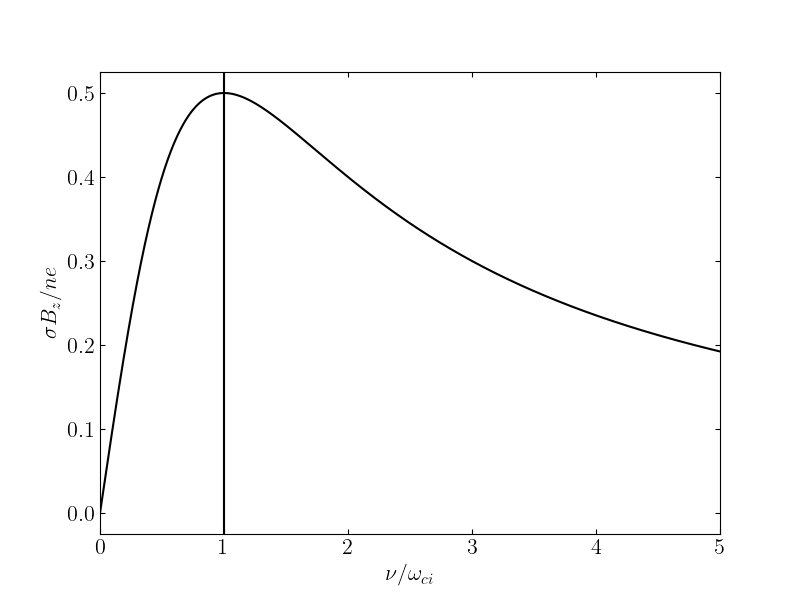
\includegraphics[width=0.7\textwidth]{p2.png}
\end{center}
The maximum satifies
\begin{equation}
    \frac{\partial
    \sigma}{\partial\nu_\text{in}}\sim\frac1{\nu_\text{in}^2+\omega_{ci}^2}-\frac{2\nu_\text{in}^2}{(\nu_\text{in}^2+\omega_{ci}^2)^2}=0 
    \Rightarrow \nu_\text{in}^2+\omega_{ci}^2-2\nu_\text{in}^2=0\Leftrightarrow
    \nu_\text{in}=\omega_{ci}
\end{equation}
This is consistent with the peak in the plot (vertical line).
\end{solution}
\end{problem}
%%%%%%%%%%%%%%%%%%%%%%%%%%%%%%%%%%%%%%%%%%%%%%%%%%%%%%%%%%%%%%%%%%%%%%%%%%%%%%%
%%%%%%%%%%%%%%%%%%%%%%%%%%%%%%%%%%%%%%%%%%%%%%%%%%%%%%%%%%%%%%%%%%%%%%%%%%%%%%%
\begin{problem}{3}[Oblique slow mode]
At oblique angles, plasmas have three characteristic modes that are
distinguished by the role of the magnetic field. We want to derive the slow mode
with $\vb{k}$ at an arbitrary angle to $\vb{B}_0$ in a strongly magnetized
plasma. The slow mode is dominated by particle pressure and, since the plasma is
strongly magnetized, there should be only a small perturbation in $\vb{B}$.
Start with our linearized wave equations
\begin{subequations}
    \begin{align}
        \omega\rho_1&=\rho_0\vb{k}\vdot\vb{u}_1\label{p3:1}\\
        \omega\rho_0\vb{u}_1&=\vb{k}\frac{\gamma T}{m}\rho_1
        +\vb{k}\frac{\qty(\vb{B}_0\vdot\vb{B}_1)}{\mu_0}
        -\frac{\qty(\vb{k}\vdot\vb{B}_0)}{\mu_0}\vb{B}_1\label{p3:2}\\
        \omega\vb{B}_1&=\vb{B}_0\qty(\vb{k}\vdot\vb{u}_1)-\qty(\vb{k}\vdot\vb{B}_0)\vb{u}_1\label{p3:3}
    \end{align} 
\end{subequations}
Let $\vb{B}_0=B_0\zhat$, $\vb{k}=k(\sin\theta\xhat+\cos\theta\zhat)$, and
$\vb{u}_1=u_1\qty(\sin\phi\xhat+\cos\phi\zhat)$. Careful! An oblique wave is
neither longitudinal nor transverse.

(a) Examine \eqref{p3:3}. If $\vb{B}_1$ is small, what is the angle $\phi$ from
$\vb{B}_0$ is $\vb{u}_1$? Remember, $\theta$ is arbitrary. Show that $\vb{u}_1$
must be nearly parallel to $\vb{B}_0$.

(b) In \eqref{p3:2}, one can immediately see that there is no solution for large
$\theta$ if $\vb{B}_1$ is exactly 0. As a rough approximation, take the dot
product of \eqref{p3:2} with $\vb{B}_0$ to derive a dispersion relation for
the oblique sound wave. Assume $\phi=0$ but $\theta$ is arbitrary after the dot
product.

(c) Now let's do the problem more accurately. Start with \eqref{p3:3} and
separate it into the $x$ and $z$ components.

(d) Next, evaluate \eqref{p3:2} in the $x$ direction. Show that $u_{1x}$ depends
on two terms; one is proportional to $c_s^2$ (sound speed) and the other is
proportional to $V_A^2$ (Alfvén speed). Show that if $V_A^2\gg c_s^2$, then
$\abs{\phi}\ll\abs{\theta}$, so our simple derivation is correct. Hint: Do not 
try to solve this problem exactly!
\begin{solution}
(a) If $\vb{B}_1$ is small, then the LHS is $\sim\vb{0}$ and we can write
$\vb{u}_1\propto\vb{B}_0$. So $\phi$ must be close to zero. In other words,
$\vb{u}_1$ is nearly parallel to $\vb{B}_0$.

(b) Taking the dot product with $\vb{B}_0$, we get
\begin{align}
    &&\omega\rho_0(\vb{u}_1\vdot\vb{B}_0)
    &=c_s^2\rho_1(\vb{k}\vdot\vb{B}_0)+\frac{(\vb{B}_0\vdot\vb{B}_1)(\vb{k}\vdot\vb{B}_0)}{\mu_0}
    -\frac{(\vb{k}\vdot\vb{B}_0)(\vb{B}_0\vdot\vb{B}_1)}{\mu_0}\notag\\
    &\Rightarrow& \omega\rho_0B_0u_1\cos\phi&=c_s^2\rho_1kB_0\cos\theta\notag\\
    &\Leftrightarrow&\frac{\omega}{k}&=c_s^2\frac{\rho_1}{\rho_0u_1}\cos\theta
\end{align}
where $\phi=0$. But from \eqref{p3:1}, we can also write $(\rho_1/\rho_0u_1)=(k/
\omega)\cos\theta$. Plugging this in, we get the dispersion relation
\begin{equation}
    \omega=kc_s\cos\theta=k_\|c_s
\end{equation}

(c) Separating \eqref{p3:3} into $x$ and $z$, we get
\begin{equation}
    \omega B_{1x}=-B_0k_zu_x\qquad\text{and}\qquad
    \omega B_{1z}=B_0(k_xu_x+k_zu_z)-B_0k_zu_z=B_0k_xu_x
\end{equation}

(d) Then the $x$ component of \eqref{p3:2} is
\begin{align}
    &&\omega\rho_0u_x
    &=\rho_1k_xc_s^2+k_x\frac{B_0B_{1z}}{\mu_0}-\frac{k_zB_0}{\mu_0}B_{1x}\notag\\
    &\Rightarrow&
    u_x&=\frac{\rho_1}{\rho_0}\frac{k_x}{\omega}c_s^2+\frac{k_x}{\omega}\frac{B_0}{\mu_0\rho_0}B_{1z}-\frac{k_z}{\omega}\frac{B_0}{\mu_0\rho_0}B_{1x}\notag\\
       &&
       &=\frac{k_x}{\omega^2}(k_xu_x+k_zu_z)c_s^2+\frac{k_x^2}{\omega^2}V_A^2u_x+\frac{k_z^2}{\omega^2}V_A^2u_x
\end{align}
Then we can solve for
\begin{equation}
    \frac{u_x}{u_z}=\tan\phi=\frac{k_xk_zc_s^2}{\omega^2-k_x^2c_s^2-k^2V_A^2} 
\end{equation}
Thus, when $c_s^2\ll V_A^2$, $\tan\phi\to0$, which means $\phi\to0$.
\end{solution}
\end{problem}
%%%%%%%%%%%%%%%%%%%%%%%%%%%%%%%%%%%%%%%%%%%%%%%%%%%%%%%%%%%%%%%%%%%%%%%%%%%%%%%
%%%%%%%%%%%%%%%%%%%%%%%%%%%%%%%%%%%%%%%%%%%%%%%%%%%%%%%%%%%%%%%%%%%%%%%%%%%%%%%
\begin{problem}{4}[Force free current sheet]
Assume a current $\vb{J}$ in the $(yz)$ plane that flows along $\vb{B}$ (also in
the $(yz)$ plane). The only gradients are in the $x$ direction. There is no
external magnetic field. For boundary conditions
\begin{equation}
    \vb{B}(x\to\infty)=-B_0\zhat,\qquad
    \vb{B}(x\to-\infty)=B_0\zhat,\qquad
    \vb{J}(x\to\pm\infty)=0
\end{equation}

(a) Find a solution for $\vb{B}$ with $\alpha=\alpha_0\sech(x/x_0)$, where $x_0$
is a ``characteristic'' of the thickness of the current sheet. Sketch $B_y,B_z$.
Sketch or describe the magnetic pressure. There are several possible solutions.
Choose the simplest one. Hint: Let $\alpha_0=1/x_0$.

(b) Compare this solution to that of a Harris current sheet (do not derive again
-- use the results from homework). Discuss the similarities and differences.
\begin{solution}
(a) As per the hint, let $\alpha=(1/x_0)\sech(x/x_0)$. Force free current sheet
satisfies
\begin{equation}
    \curl{\vb{B}}=\mu_0\vb{J}=\alpha\vb{B} 
\end{equation}
Thus, the magnetic field components satisfy the following system of differential
equations
\begin{equation}
    \frac{\partial B_z}{\partial x}=-\alpha B_y\qquad\text{and}\qquad
    \frac{\partial B_y}{\partial x}=\alpha B_z
\end{equation}
Taking another $x$ derivative and combining the two equations, we get the
following differential equation in $B_z$
\begin{equation}
    \frac{\partial^2B_z}{\partial
    x^2}+\frac1{x_0}\tanh(\frac{x}{x_0})\frac{\partial B_z}{\partial
x}+\frac1{x_0^2}\sech^2\qty(\frac{x}{x_0})B_z=0 
\end{equation}
The general solution is obtained from Mathematica
\begin{equation}
    B_z=\frac{c_1}{\cosh(x/x_0)}+c_2\tanh\qty(\frac{x}{x_0}) 
\end{equation}
with $c_1,c_2$ constants. Now, we can let $c_1=0$ and $c_2=-B_0$ so that $B_z$
matches the boundary conditions. It follows that
\begin{equation}
    B_y=-\frac1{\alpha}\frac{\partial B_z}{\partial x}=B_0\sech(\frac{x}{x_0}) 
\end{equation}
In full, the magnetic field is
\begin{equation}
    \vb{B}=B_0\qty[\sech\qty(\frac{x}{x_0})\yhat-\tanh\qty(\frac{x}{x_0})\zhat] 
\end{equation}
and the current is
\begin{equation}
    \vb{J}=\frac{\alpha}{\mu_0}\vb{B}=\frac{B_0}{\mu_0x_0}\sech(\frac{x}{x_0})\qty[\sech\qty(\frac{x}{x_0})\yhat-\tanh\qty(\frac{x}{x_0})\zhat] 
\end{equation}
So $\vb{J}(x\to\pm\infty)=0$. This also matches the boundary conditions. In the
following, we plot the components $B_y$ (red), $B_z$ (blue), and the normalized
magnetic pressure $(B^2/2\mu_0)/(B_0^2/2\mu_0)$ (black).
\begin{center}
    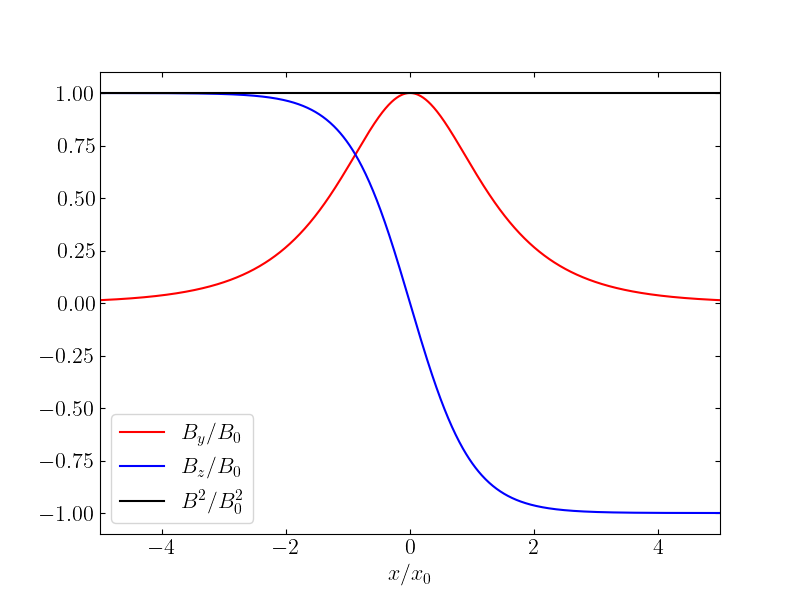
\includegraphics[width=0.8\textwidth]{p4.png}
\end{center}

(b) The magnetic pressure is constant here, but not in the Harris
current sheet. $B_z$ has the same shape as that in the Harris current sheet. 
However, $B_y$ is non-zero here. Similarly, $J_y$ has the same shape as that in
the Harris current sheet, but $J_z$ is non-zero here.
\end{solution}
\end{problem}
%%%%%%%%%%%%%%%%%%%%%%%%%%%%%%%%%%%%%%%%%%%%%%%%%%%%%%%%%%%%%%%%%%%%%%%%%%%%%%%    
%%%%%%%%%%%%%%%%%%%%%%%%%%%%%%%%%%%%%%%%%%%%%%%%%%%%%%%%%%%%%%%%%%%%%%%%%%%%%%%
\begin{problem}{5}[Isothermal shock]
In some astrophysical situations, radiative cooling is so efficient that the
post-shock temperature relaxes to the pre-shock temperature within a thin layer.
Under this rare condition, the shock can be treated isothermal. In this problem,
we derive the compression ratio for a perpendicular isothermal shock.

(a) Show the energy equation for a perpendicular isothermal shock in the limit
$\gamma\to1$ is: $u_1P_1=u_2P_2$.

(b) Write down the remaining jump conditions for a perpendicular isothermal
shock.

(c) Eliminate $\rho_2,u_2,P_2$, and $B_2$ from the equation for the pressure
balance. The result should only have $\rho_1,u_1,P_1,B_1$, and the compression
ratio $r=\rho_2/\rho_1$.

(d) Remove the trivial solution ($r=1$) by dividing by $1-r$. You should arrive
at a quadratic equation in $r$ (you may have to multiply by $r$).

(e) Solve for the compression ratio $r$ as a function of $u_1$ in the limit of
high Alfvén Mach isothermal shock. Hint: you do not need to solve the quadratic
equation. Reform the equation in terms of $M_A$ and $M_S$ and assume $M_A\gg 1$.

(f) Now solve for the compression ratio as a function of $u_1$ for $B=0$. How
does this solution differ from the magnetized case?

(g) Briefly discuss the effect of a finite magnetic field in high-Mach
isothermal shock.
\begin{solution}
(a) The energy equation for a perpendicular shock is, ignoring the ram energy
and magnetic field energy
\begin{equation}
    \frac{\gamma}{\gamma-1}u_1P_1=\frac{\gamma}{\gamma-1}u_2P_2 
\end{equation}
Using l'Hôpital's rule, both $\gamma/(\gamma-1)\to1$ when $\gamma\to1$. So we
get $u_1P_1=u_2P_2$.

(b) The remaining jump conditions are
\begin{subequations}
    \begin{align}
        \rho_1u_1&=\rho_2u_2\\
        u_1B_1&=u_2B_2\\
        P_1+\rho_1u_1^2+\frac{B_1^2}{2\mu_0}&=P_2+\rho_2u_2^2+\frac{B_2^2}{2\mu_0}\label{p5b:P}
    \end{align} 
\end{subequations}

(c,d) From \eqref{p5b:P}, we can write
\begin{align}\label{p5c}
    &&P_1\qty(1-\frac{P_2}{P_1})+\rho_1u_1^2\qty(1-\frac{\rho_2}{\rho_1}\frac{u_2^2}{u_1^2})+\frac{B_1^2}{2\mu_0}\qty(1-\frac{B_2^2}{B_1^2})&=0\notag\\
    &\Rightarrow&
    P_1(1-r)+\rho_1u_1^2\qty(1-\frac1r)+\frac{B_1^2}{2\mu_0}\qty(1-r^2)&=0\notag\\
    &\Leftrightarrow&
    rP_1-\rho_1u_1^2+\frac{B_1^2}{2\mu_0}\qty(r+r^2)&=0
\end{align}

(e) Dividing \eqref{p5c} by $\rho_1u_1^2$, we get
\begin{equation}
    \frac{r}{M_S^2}-1+\frac{r+r^2}{2M_A^2}=0 
\end{equation}
For $M_A\gg 1$, the quadratic term vanishes and we can write
$r=M_S^2=(\rho_1/P_1)u_1^2$.

(f) In the unmagnetized case, \eqref{p5b:P} becomes
\begin{equation}
    P_1+\rho_1u_1^2=P_2+\rho_2u_2^2 
\end{equation}
Similarly, we eliminate $P_2,\rho_2,u_2$
\begin{equation}
    P_1\qty(1-\frac{P_2}{P_1})+\rho_1u_1^2\qty(1-\frac{\rho_2}{\rho_1}\frac{u_2^2}{u_1^2})=P_1(1-r)+\rho_1u_1^2\qty(1-\frac1r)=0 
\end{equation}
Dividing by $\rho_1u_1^2$ yields
\begin{equation}
    \frac{1}{M_S^2}-\frac1r=0\Rightarrow r=M_S^2=\frac{\rho_1}{P_1}u_1^2
\end{equation}

(g) So a finite magnetic field has no effect on an isothermal shock.
\end{solution}
\end{problem}
%%%%%%%%%%%%%%%%%%%%%%%%%%%%%%%%%%%%%%%%%%%%%%%%%%%%%%%%%%%%%%%%%%%%%%%%%%%%%%%
\end{document}
